% ****** Start of file apssamp.tex ******
%
%   This file is part of the APS files in the REVTeX 4.2 distribution.
%   Version 4.2a of REVTeX, December 2014
%
%   Copyright (c) 2014 The American Physical Society.
%
%   See the REVTeX 4 README file for restrictions and more information.
%
% TeX'ing this file requires that you have AMS-LaTeX 2.0 installed
% as well as the rest of the prerequisites for REVTeX 4.2
%
% See the REVTeX 4 README file
% It also requires running BibTeX. The commands are as follows:
%
%  1)  latex apssamp.tex
%  2)  bibtex apssamp
%  3)  latex apssamp.tex
%  4)  latex apssamp.tex
%
\documentclass[%
 preprint,
%superscriptaddress,
%groupedaddress,
%unsortedaddress,
%runinaddress,
%frontmatterverbose, 
%preprint,
%preprintnumbers,
%nofootinbib,
%nobibnotes,
%bibnotes,
 amsmath,amssymb,
 aps,
%pra,
%prb,
%rmp,
%prstab,
%prstper,
%floatfix,
]{revtex4-2}

\usepackage{graphicx}% Include figure files
\usepackage{dcolumn}% Align table columns on decimal point
\usepackage{bm}% bold math
\usepackage{float}
%\usepackage{hyperref}% add hypertext capabilities
%\usepackage[mathlines]{lineno}% Enable numbering of text and display math
%\linenumbers\relax % Commence numbering lines

%\usepackage[showframe,%Uncomment any one of the following lines to test 
%%scale=0.7, marginratio={1:1, 2:3}, ignoreall,% default settings
%%text={7in,10in},centering,
%%margin=1.5in,
%%total={6.5in,8.75in}, top=1.2in, left=0.9in, includefoot,
%%height=10in,a5paper,hmargin={3cm,0.8in},
%]{geometry}

\begin{document}

\preprint{APS/123-QED}

\title{Spiral unpinning in BZ reaction via forced retardation with a rotating electric field }% Force line breaks with \\


\author{Amrutha S V}
\thanks{equal contribution}% 
\author{Anupama Sebastian}%

\author{P P Sibeesh}

\author{T K Shajahan}
\affiliation{
 Dpeartment of Physics\\ National Institute of Technology Karnataka}
 \email{shajahantk@nitk.edu.in}


\date{\today}% It is always \today, today,
             %  but any date may be explicitly specified

\begin{abstract}
The mechanism of spiral wave unpinning in the BZ reaction with an applied rotating electric field is investigated by varying the pacing ratio, initial spiral phase, and field strength. Forced retardation of the pinned spiral wave by the electric field, while propagating away from the anode, induces unpinning. The unpinning occurs within the limits of the unpinning phase window calculated using the derived analytical formulae. The experimental observations are verified using the numerical simulations performed with the Oregonator model.
\vspace{5pt}
\hrule
\vspace{5pt} 
\end{abstract}

%\keywords{Suggested keywords}%Use showkeys class option if keyword
                              %display desired
                             
\maketitle

%\tableofcontents

%\section{Introduction}

Chemical waves in the oscillating BZ reaction are being studied intensively because of their applicability in various interdisciplinary areas, including the chemical computing~\cite{gorecki2022information} and the self-propelled motion~\cite{jin2017chemotaxis, ryabchun2022run}. The BZ reaction models the excitable media~\cite{sinha2014patterns}. Thin layers of the BZ reaction exhibit spatio-temporal patterns such as expanding target waves~\cite{zhang2019stability} or rotating spiral waves~\cite{zykov2018spiral}. The tip of a rotating spiral wave can pin to inhomogeneities present in the medium. Pinning alters the wave parameters such as the wave period, wavelength, and velocity depending on the size of the pinning obstacle~\cite{lim2006spiral, sutthiopad2015propagation}. An applied electric field can achieve unpinning of pinned spirals from the inhomogeneities~\cite{jimenez2013electric,punacha2020theory}. 
Application of external electric field to the excitable systems, especially to the chemical and biological systems, can have a sensitive control over the wave dynamics~\cite{steinbock1992electric,bittihn2012negative,feng2022removal}.

Field-induced unpinning of spiral waves in excitable cardiac tissue occurs due to the secondary wave emission~\cite{pumir2007wave} from the pinning obstacle. However, an applied electric field does not induce wave emission in the BZ reaction. The variations in the chemical wave dynamics in an applied electric field are correlated with the oriented movement of ionic species in the medium.
So the mechanism of spiral unpinning is quite different in the chemical excitable medium. A slowdown in the spiral velocity due to the electric force leads to unpinning of a pinned spiral tip in a DC electric field~\cite{dcmechanism}. In such cases, the field is static. But in a rotating electric field, the spiral and the field rotate with specific frequencies.
Numerical studies in reaction-diffusion models show that a rotating CPEF can synchronize the spiral frequency~\cite{chen2009synchronization} and make a chiral selection~\cite{li2013chiral}.
A co-rotating CPEF can induce a maximum spiral drift, but a counter-rotation locks the drift~\cite{chen2006drift}. Unpinning of two~\cite{punacha2020theory} and three-dimensional~\cite{pan2016removal} vortices is also reported in the cardiac models using the CPEF. The only experimental study of CPEF in the BZ reaction is reported by Ji et al. \cite{ji2013experimental}. 
The control of spiral turbulence obtained in the BZ reaction with CPEF is explained based on frequency synchronization. 
 
In this paper, for the first time to our knowledge, the unpinning of a spiral wave with the circularly polarised electric field (CPEF) in the BZ reaction is reported. We will address the mechanism of spiral unpinning and formulate it analytically.
 
\vspace{5pt}
\hrule
\vspace{5pt}


Our experiments were carried out in a ferroin-catalyzed BZ reaction with the following initial reagent concentrations: [$H_2SO_4$] = 0.16 M, [$NaBrO_3$] = 40 mM, [Malonic acid] = 40 mM, and [Ferroin] = 0.5 mM. The reaction mixture is embedded in 1.4 $\%$ w/v of agar gel to avoid any hydrodynamic perturbations. The single reaction layer of thickness $3$ mm is taken in a glass petri dish of diameter $10$ cm. 
A circular excitation wave is created at the center of the reaction medium by inserting a silver wire. By disrupting the motion of the circular wavefront, a pair of counter-rotating spirals are created. A glass bead of diameter $1.2$ mm is carefully placed at the tip of one of the spirals. The pinning of the spiral tip to the obstacle is confirmed after 1-2 rotations.
An anticlockwise rotating circularly polarized electric field (CPEF) is applied using two pairs of copper electrodes as in FIG.1. 

Images of the reaction medium are recorded using a CCD camera at every $30 s$ interval for $1-2$ hours. Even though the results contain only the unpinning of a spiral pinned to a spherical bead, a comparative study with a spiral pinned to a cylindrical rod is included in the appendix (see appendix).

\vspace{5pt}
\hrule
\vspace{5pt}

From a mathematical point of view, the dynamical features of the BZ reaction can be described using the Oregonator model. 

\begin{equation}\label{E_uoregonator}
\frac{\partial u}{\partial t}=\frac{1}{\epsilon}(u(1-u)-\frac{fv(u-q)}{u+q})
+D_{u}\nabla^2u+M_{u}(\vec{E} \cdot \nabla u)
\end{equation}
\begin{equation}\label{E_voregonator}
\frac{\partial v}{\partial t}=u-v+D_{v}\nabla^2v+M_{v}(\vec{E} \cdot \nabla v).
\end{equation}

Here, $u$ is the activator variable, and $v$ is the inhibitor variable (corresponding to the rescaled concentrations of [HBrO2] and the catalyst, respectively). $\vec{E} = E_{0} sin(\frac{2\pi t}{T})\hat{x} + E_{0} cos(\frac{2\pi t}{T})\hat{y}$ is the circularly polarized electric field. The electric field is added as an advection term for the variables $u$ and $v$. 

The model parameters are $q = 0.002$, $f = 1.4$ and $\epsilon=0.04$. The diffusion coefficients are $D_{u}=1.0$ and $D_{v}=0.6$. $M_{u}=1.0$ and $M_{v}=-2.0$ are the ionic mobilities of $u$ and $v$ respectively. The computation domain of size $300 \times 300$ is discretized into grids of uniform size $dx=dy=0.1$ (s.u) in space. The explicit forward Euler method with a time step, $dt=0.0001$, is used to study the time evolution. No-flux boundary conditions are imposed both on the domain and obstacle boundary. An obstacle of radius, $r = 10$ s.u, is created at the center of the domain by reducing the value of $D_{u}=0.0001$ inside the obstacle. Phase-field method is used to set no-flux boundary conditions at the obstacle boundary \cite{fenton2005modeling}. 
All the numerical results shown in this paper are carried out with the two-variable Oregonator model. But in the appendix, the results obtained from a three-variable Oregonator model are compared with those obtained from the two-variable model, and both show good agreement (see the Appendix).
 

\vspace{5pt}
\hrule
\vspace{5pt}

%\section{Results and Discussions}

The location of the spiral tip on the obstacle is denoted by its phase, $\phi_s$. The spiral phase at t = 0 s is represented as $\phi_0$ (initial spiral phase), and the phase at the time of unpinning is $\phi_u$ (unpinning phase). $\phi_s$ is measured anti-clockwise from the positive X-axis in degree by considering the obstacle center as the origin.
The direction of the spiral tip rotation ($\hat{r_t}$) can be obtained by drawing a tangent at the respective phases. In experiments, $\phi_s$ is determined from the images using the software GIMP~\cite{gimp}.
The resolution in angle measurements is 6.67$^0$ for a bead of diameter 1.2 mm.
%Experimental images have a resolution of 0.07 mm/pixel.
In simulations, the point of intersection of the two contours
$u=1/2$ and $F(1/2,v) = 0$  is defined as the spiral tip. Here, $F$ is given by the reaction term in the equation 
(\ref{E_uoregonator})\cite{barkley1991model}.

%%%%%%%%%%%%%%%%%%%%%%%%%%%%%%%%%%%%%%%%%%%%%%%%%%%%%%%%%%%%%%%%%%%%%%%%%%%%%%%%%%%%%%%%%%%%%%%%%%%%%%%%%%%%%%%%%

\begin{figure}[H]
    \centering
    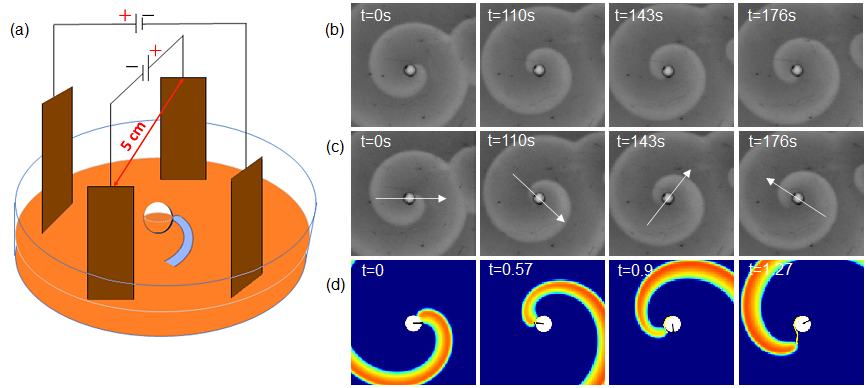
\includegraphics[scale=0.7]{new_fig.png}
    \caption{\textbf{(a) Schematic diagram of the experimental system:} The positions of two pairs of field electrodes with respect to the glass bead are shown schematically (not to scale).
    \textbf{Unpinning of an anti-clockwise rotating spiral using CPEF:}  (b) An ACW rotating spiral pinned to a spherical bead of diameter 1.2 mm in the experiment. The natural period of pinned spiral tip $T_{s} = 297 $ s. (c) A CPEF of strength $E_0 \simeq 1.38$ V/cm, and period $T_{E} = 125$ s applied to the medium unpins the spiral tip from the obstacle. 
    (d) An ACW rotating spiral pinned to an obstacle of diameter 1.0 s.u in the simulation with $T_{s} = 1.77$ t.u is subjected to a CPEF of strength $E_0 \simeq 0.6 $ and period $T_{E} =1.18$ t.u. The spiral tip unpins from the obstacle at t = 1.27 t.u.
    The arrows show the direction of the applied CPEF.}
    \label{fig:unpinning_images}
\end{figure}
 
As in the DC electric field [cite], the spiral can be unpinned with the CPEF only when the field strength E equals a certain threshold value $E_{th}$. The major difference from the DC electric field is that the field is static there, but here it is rotating.
Fig.\ref{fig:unpinning_images}b gives the time sequence of field-free rotation of an ACW spiral wave and its unpinning with a CPEF of strength $E = E_{th}$. 
In experiments, the ACW spiral rotates with a period $T_{s} = 297 s$ and the period of the applied field is $T_{E} = 125 s$. In simulations, $T_{s} = 1.77$ t.u and $T_{E} =1.18$ t.u. In both cases, the spiral rotates with a lower frequency than the field ($T_{s} > T_{E}$). Hence, we say the pacing is overdrive. The ratio between the time periods of the spiral and the field rotation is denoted as the pacing ratio; $p = T_{s}/T_{E}$. In terms of angular displacements,
\begin{equation}
p = \frac{\theta_{E} - \theta_{0}}{\phi_{s} - \phi_{0}}
\label{p_theta_phi}
\end{equation}
where $\theta_{0} = 0^0$ and $\theta_{E}$ is the angle covered by the field vector by the time of unpinning.

From Fig.\ref{fig:unpinning_images}c and Fig.\ref{fig:unpinning_images}d, it can be seen that the unpinning is initiated as the spiral start to rotate towards the cathode after passing the anode. 
In Fig.\ref{fig:unpinning_images}b, at t = 110 s, if we mark $\hat{r_t}$, it will align parallel to the field vector $\vec{E}$. So the electric force on the spiral will be in the opposite direction to $\hat{r_t}$, and hence its speed reduces. If the applied field strength is equal to $E_{th}$, this reduction in the speed of spiral rotation leads to unpinning of the tip from the obstacle. This condition is similar to the unpinning at $E_{th}$ in a DC electric field~\cite{dcmechanism}. Fig.\ref{fig:acw_theory} schematically represents the above-explained mechanism of spiral unpinning in a CPEF. 

\begin{figure}[H]
    \centering
    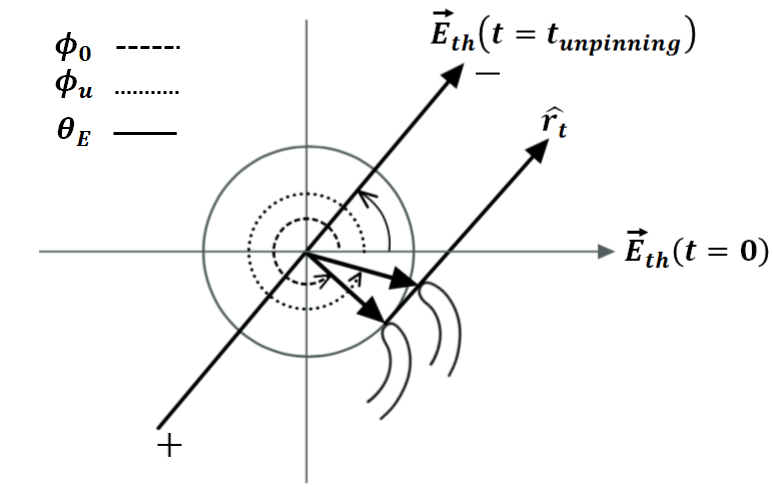
\includegraphics[width=0.8\linewidth]{theory.png}
    \caption{Schematic diagram showing the mechanism of unpinning at $E=E_{th}$: $\phi_{0}$ and  $\phi_{u}$ are the phase of the spiral tip at $t=0$ and at the time of unpinning respectively. $\theta_{E}$ denotes the phase of the electric field ${\vec{E}}$ and ${\hat{r}}_{t}$ is the tangential vector of spiral rotation on the obstacle boundary. All phases are measured in the anticlockwise direction from the initial direction of the $\vec{E}$ field. The wave unpins when the electric force is opposite to $\hat{r_t}$ (or when ${\vec{E}}$ and ${\hat{r}}_{t}$ are parallel to each other).
    }
    
    \label{fig:acw_theory}
\end{figure}

%%%%%%%%%%%%%%%%%%%%%%%%%%%%%%%%%%%%%%%%%%%%%%%%%%%%%%N%%%%%%%%%%%%%%%%%%%%%%%%%%%%%%%%%%%%%%%%%%%%%%%%%%%%%%%%
So, the unpinning at $E=E_{th}$ occurs when $\vec{E}$ align parallel to $\hat{r_t}$. This condition will provide a range of $\phi_{u}$ as,
 \begin{equation}
\theta_{E} - \pi + {\sin^{-1}} (\frac{E_{th}}{E})  \leq \phi_u \leq \theta_{E}-{\sin^{-1}} (\frac{E_{th}}{E}) 
\label{eq:phiu_range}
\end{equation}
which is the same as in a static DC field~\cite{dcmechanism}. In the DC field, $\theta_{E}$ is a constant.
But, here, $\theta_{E}$ is a function of the pacing ratio and the spiral phase according to the equation.\ref{p_theta_phi}. 
By considering the rotation of both the field and the spiral, at E=$E_{th}$ equation.\ref{eq:phiu_range} reduces to, 

\begin{subequations}
\begin{align}
\phi_u = \frac{p \phi_0+ 90}{p-1} ; p>1 \\
\phi_u = \frac{270-p \phi_0}{1-p} ; p<1  
\end{align}
\label{eq:Eth}
\end{subequations}

Figure.\ref{fig:unpinning_Eth}a and Figure.\ref{fig:unpinning_Eth}b show the variations in the values of $\Delta\phi_s = \phi_u - \phi_0$ with p obtained in experiments and simulations, respectively. The values agree with the theoretical predictions according to equation.\ref{eq:Eth}a and \ref{eq:Eth}b (solid line). 

\begin{figure}[H]
    \centering
    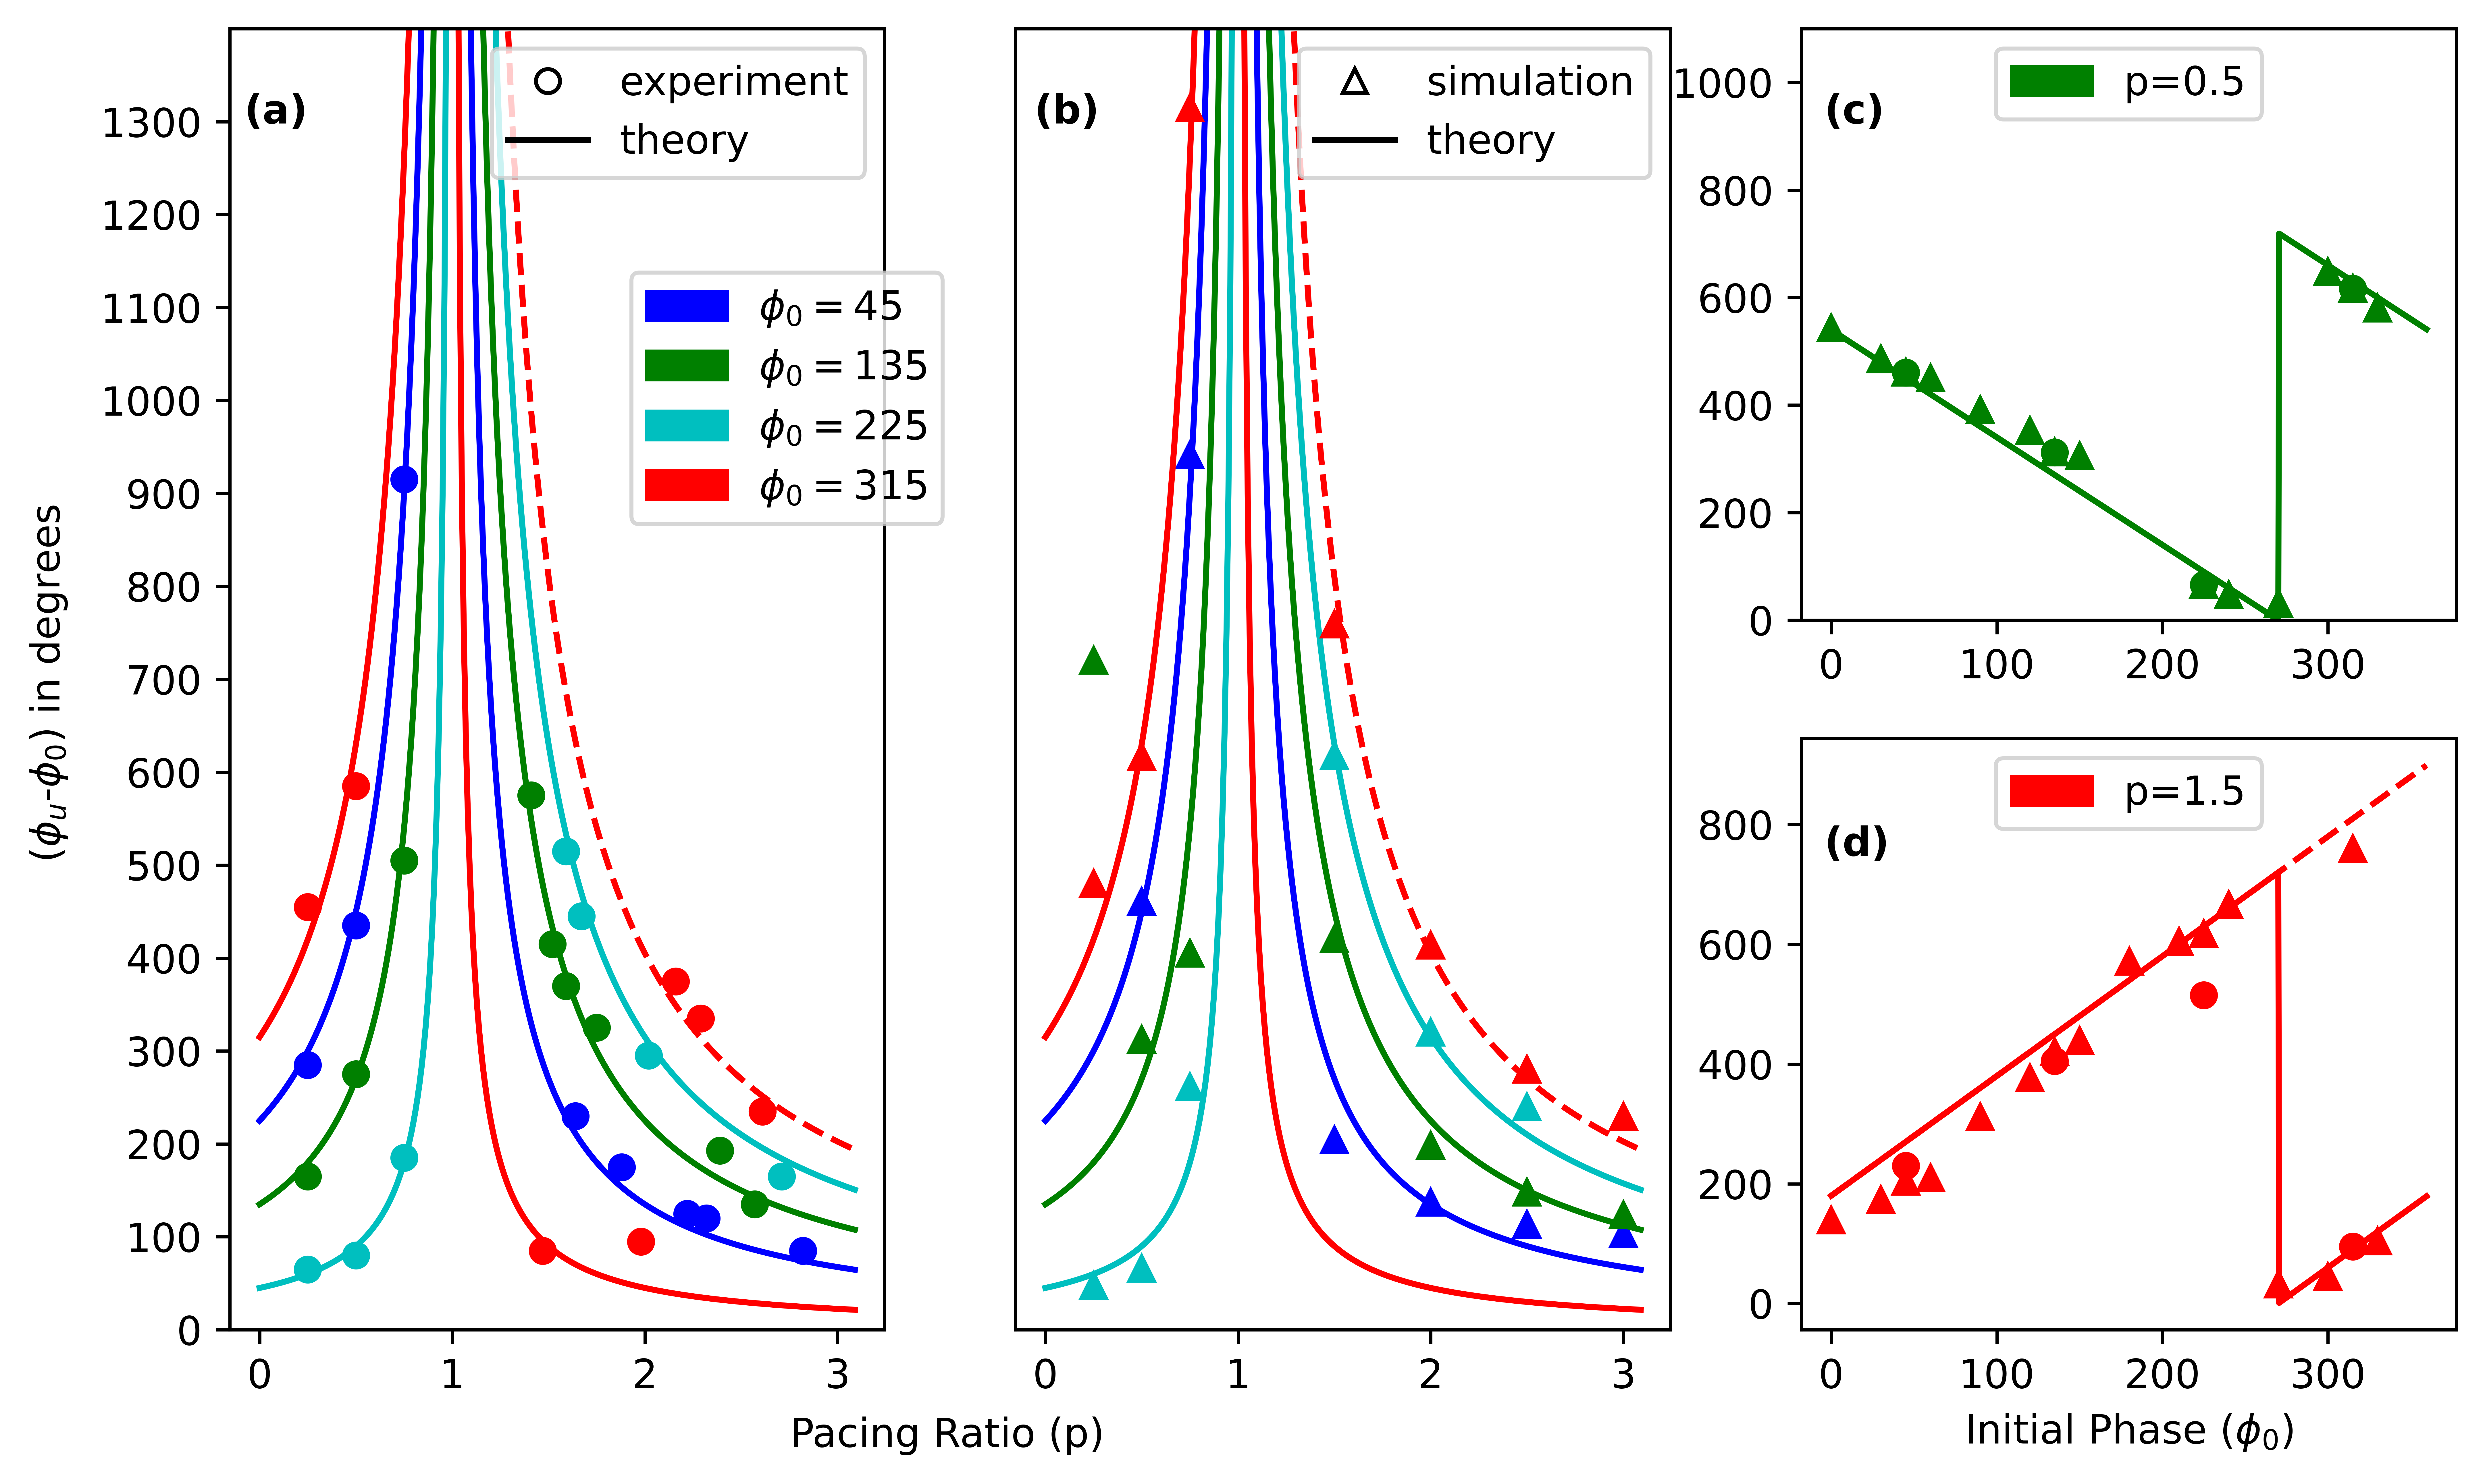
\includegraphics[scale=0.7]{Fig2.png}
    \caption{\textbf{Unpinning at $E = E_{th}$:} For spirals having different ${\phi}_0$,  the phase difference (${\phi}_u$- ${\phi}_0$) is plotted with the pacing ratio, p in (a) experiments and (b) simulations. At overdrive pacing ($p>$1), the red dashed lines on the top marks the theory curve for ${\phi}_0$=$315^0$ , corresponding to the second angular positions satisfying the unpinning mechanism. The solid red line at the bottom corresponds to the first set of angular positions satisfying the unpinning mechanism for ${\phi}_0$=$315^0$.
    (c) The phase difference (${\phi}_u$- ${\phi}_0$) is plotted against ${\phi}_0$ for $p$ = 0.5 (underdrive pacing). (d) same as (c) but for $p$ = 1.5 (overdrive pacing). The condition where our unpinning condition repeats itself a second time is indicated by the dashed line. Circles and triangles represent the experiment and simulation data respectively.  
    %Note: Remaining experimental data will be added later.
    }
    \label{fig:unpinning_Eth}
\end{figure}

The unpinning phase $\phi_{u}$ explicitly depends on the pacing ratio, p (Fig.\ref{fig:unpinning_Eth}~a,b) and the initial spiral phase, $\phi_{0}$ (Fig.\ref{fig:unpinning_Eth}~c,d). For example, in Fig.\ref{fig:unpinning_Eth}~a the spiral waves with $\phi_{0}$ = $225^0$ unpins with a minimum $\Delta\phi \simeq 50^0$ for $p<1$. %where $\Delta\phi = \phi_{u} - \phi_{0}$ is the spiral phase difference. 
But the spirals with the same initial phase unpins with a larger phase difference $\Delta\phi \simeq 150^0$ for $p>1$. At the same time, if we choose $\phi_{0} = 45^0$, the unpinning occurs quickly with $p>1$. 
The experiments and simulations showed that the unpinning is not instantaneous with the field application. Rather, it requires a minimum duration of interaction between the spiral and the field. So when the field starts with $\phi_{0}$ = $225^0$, the spiral experiences an opposite drag from the beginning itself. In low pacing, it is possible to achieve the required interaction before the tip changes its orientation. But in high pacing, the orientation changes quickly, and the process of unpinning delays comparatively. 

The variation in the unpinning phase with the initial phase is plotted in Fig.\ref{fig:unpinning_Eth}c and Fig.\ref{fig:unpinning_Eth}d by fixing the pacing ratio at 0.5 and 1.5, respectively. From the figures, it is evident that as $\phi_0$ increases from $0^0$ to $270^0$, $\phi_{u}$ decreases linearly for $p<1$ and increases linearly for $p>1$. At $\phi_{0} = 270^0$, there occurs a sudden raise or fall in $\Delta\phi$-value and at $\phi_{0} = 360^0$, $\Delta\phi$ resets to the value corresponding to $\phi_{0} = 0^0$. In Fig.\ref{fig:unpinning_Eth}a and \ref{fig:unpinning_Eth}b, there are two theoretical curves for $\phi_{u}$ corresponding to $\phi_{0}$ = $315^0$. But from the equation.\ref{eq:overdrive} at E = $E_{th}$, $\phi_{u}$ can have only a single value, represented by the solid red line at the bottom. Instead, the unpinning happened at a subsequent $\phi_{s}$ after the expected $\phi_{u}$, where the condition for unpinning is satisfied (red dashed line in Fig.\ref{fig:unpinning_Eth}~a,b). The same is marked as the dashed line in Fig.\ref{fig:unpinning_Eth}~d. Such a significant change is most probable for high pacing ratios ($p>2$). 




Following the mechanism at E = $E_{th}$, the unpinning for a field strength greater than $E_{th}$ must occur when the component of $\vec{E}$ along $\hat{r_t}$ reaches the critical threshold, $E_{th}$. i.e, when the scalar product of ${\vec{E}}$ and ${\hat{r}}_{t}$ is equal to or greater than $E_{th}$. This condition gives a window of possible spiral unpinning phase $\phi_{u}$ in terms of $\phi_{0}$, p, E and $E_{th}$ as in equation.\ref{eq:phiu_range}.

For overdrive pacing with $p>1$, the unpinning phase window is given by
\begin{equation}
\frac{p \phi_0+ {\sin^{-1}}(\frac{E_{th}}{E})}{p-1}   \leq \phi_u \leq \frac{p \phi_0+\pi -{\sin^{-1}}(\frac{E_{th}}{E})}{p-1}
\label{eq:overdrive}
\end{equation}
with a width $\Delta\phi_u = \frac{\pi - 2 \sin^{-1}(\frac{E_{th}}{E})}{p-1}$.

For underdrive pacing i.e, for $p<1$, the unpinning phase window is 
\begin{equation}
\frac{\pi+ {\sin^{-1}}(\frac{E_{th}}{E})-p \phi_0}{1-p}   \leq \phi_u \leq \frac{2\pi-p \phi_0-{\sin^{-1}}(\frac{E_{th}}{E})}{1-p}
\label{eq:underdrive}
\end{equation}
The width of this window is $\Delta\phi_u = \frac{\pi - 2 \sin^{-1}(\frac{E_{th}}{E})}{1-p}$.

%%%%%%%%%%%%%%%%%%%%%%%%%%%%%%%%%%%%%%%%%%%%%%%%%%%%%%%%%%%%%%%%%%%%%%%%%%%%%%%%%%%%%%%%%%%%%%%%%%%%%%%%
%At $E_{th}$ the above conditions reduces to a single equation and the theoretical values matches well with the numerical and experimental values (Fig.\ref{fig:unpinning_Eth}). 


%The above argument can also explain the observation of a lower $E_{th}$ value for $p<1$ (0.9 V/cm) than that for $p>1$ (1.38 V/cm).







%Every measured $\phi_u$ values comes within these limits except a few in the case of $\phi_{0} = 315^0$. 
\begin{figure}[H]
    \centering
    \includegraphics[scale=0.7]{E.png}
    \caption{\textbf{(a) Unpinning at $E>E_{th}$ for ${\phi}_0 = 225^0$ (${\sin^{-1}}{(\frac{E_{th}}{E})}=48.95^0$):} The solid bottom line represents the lower limit of the range of possible ${\phi}_u$ and the top dashed line represents the upper limit of the range of possible ${\phi}_u$ (Equation.\ref{eq:overdrive} and \ref{eq:underdrive}). The dotted yellow line represents ${\phi}_u$ at $E=E_{th}$.
    \textbf{(b) Unpinning of spiral wave with pacing ratio, p = 1 for different field strength:} $\pi+{\sin^{-1}}{(\frac{E_{th}}{E})}$ and $2\pi-{\sin^{-1}}{(\frac{E_{th}}{E})}$ are the lower and upper limit of 
    the range of possible ${\phi}_0$ which gives successful unpinning for p = 1. Shaded region corresponds to the cases of successful unpinning.
    Circles and diamonds represent the experiment and simulation data respectively.}
    \label{fig:E_p1}
\end{figure}

\iffalse
%%%%%%%%%%%%%%%%%%%%%%%%%%%%%%%%%%%%%%%%%%%%%%%%%%%%%%%%%%%%%%%%%%%%%%%%%%%%%%%%%%%%%%%%%%%%%%%%%%%%%%%%%%%%
\begin{figure}[H]
    \centering
    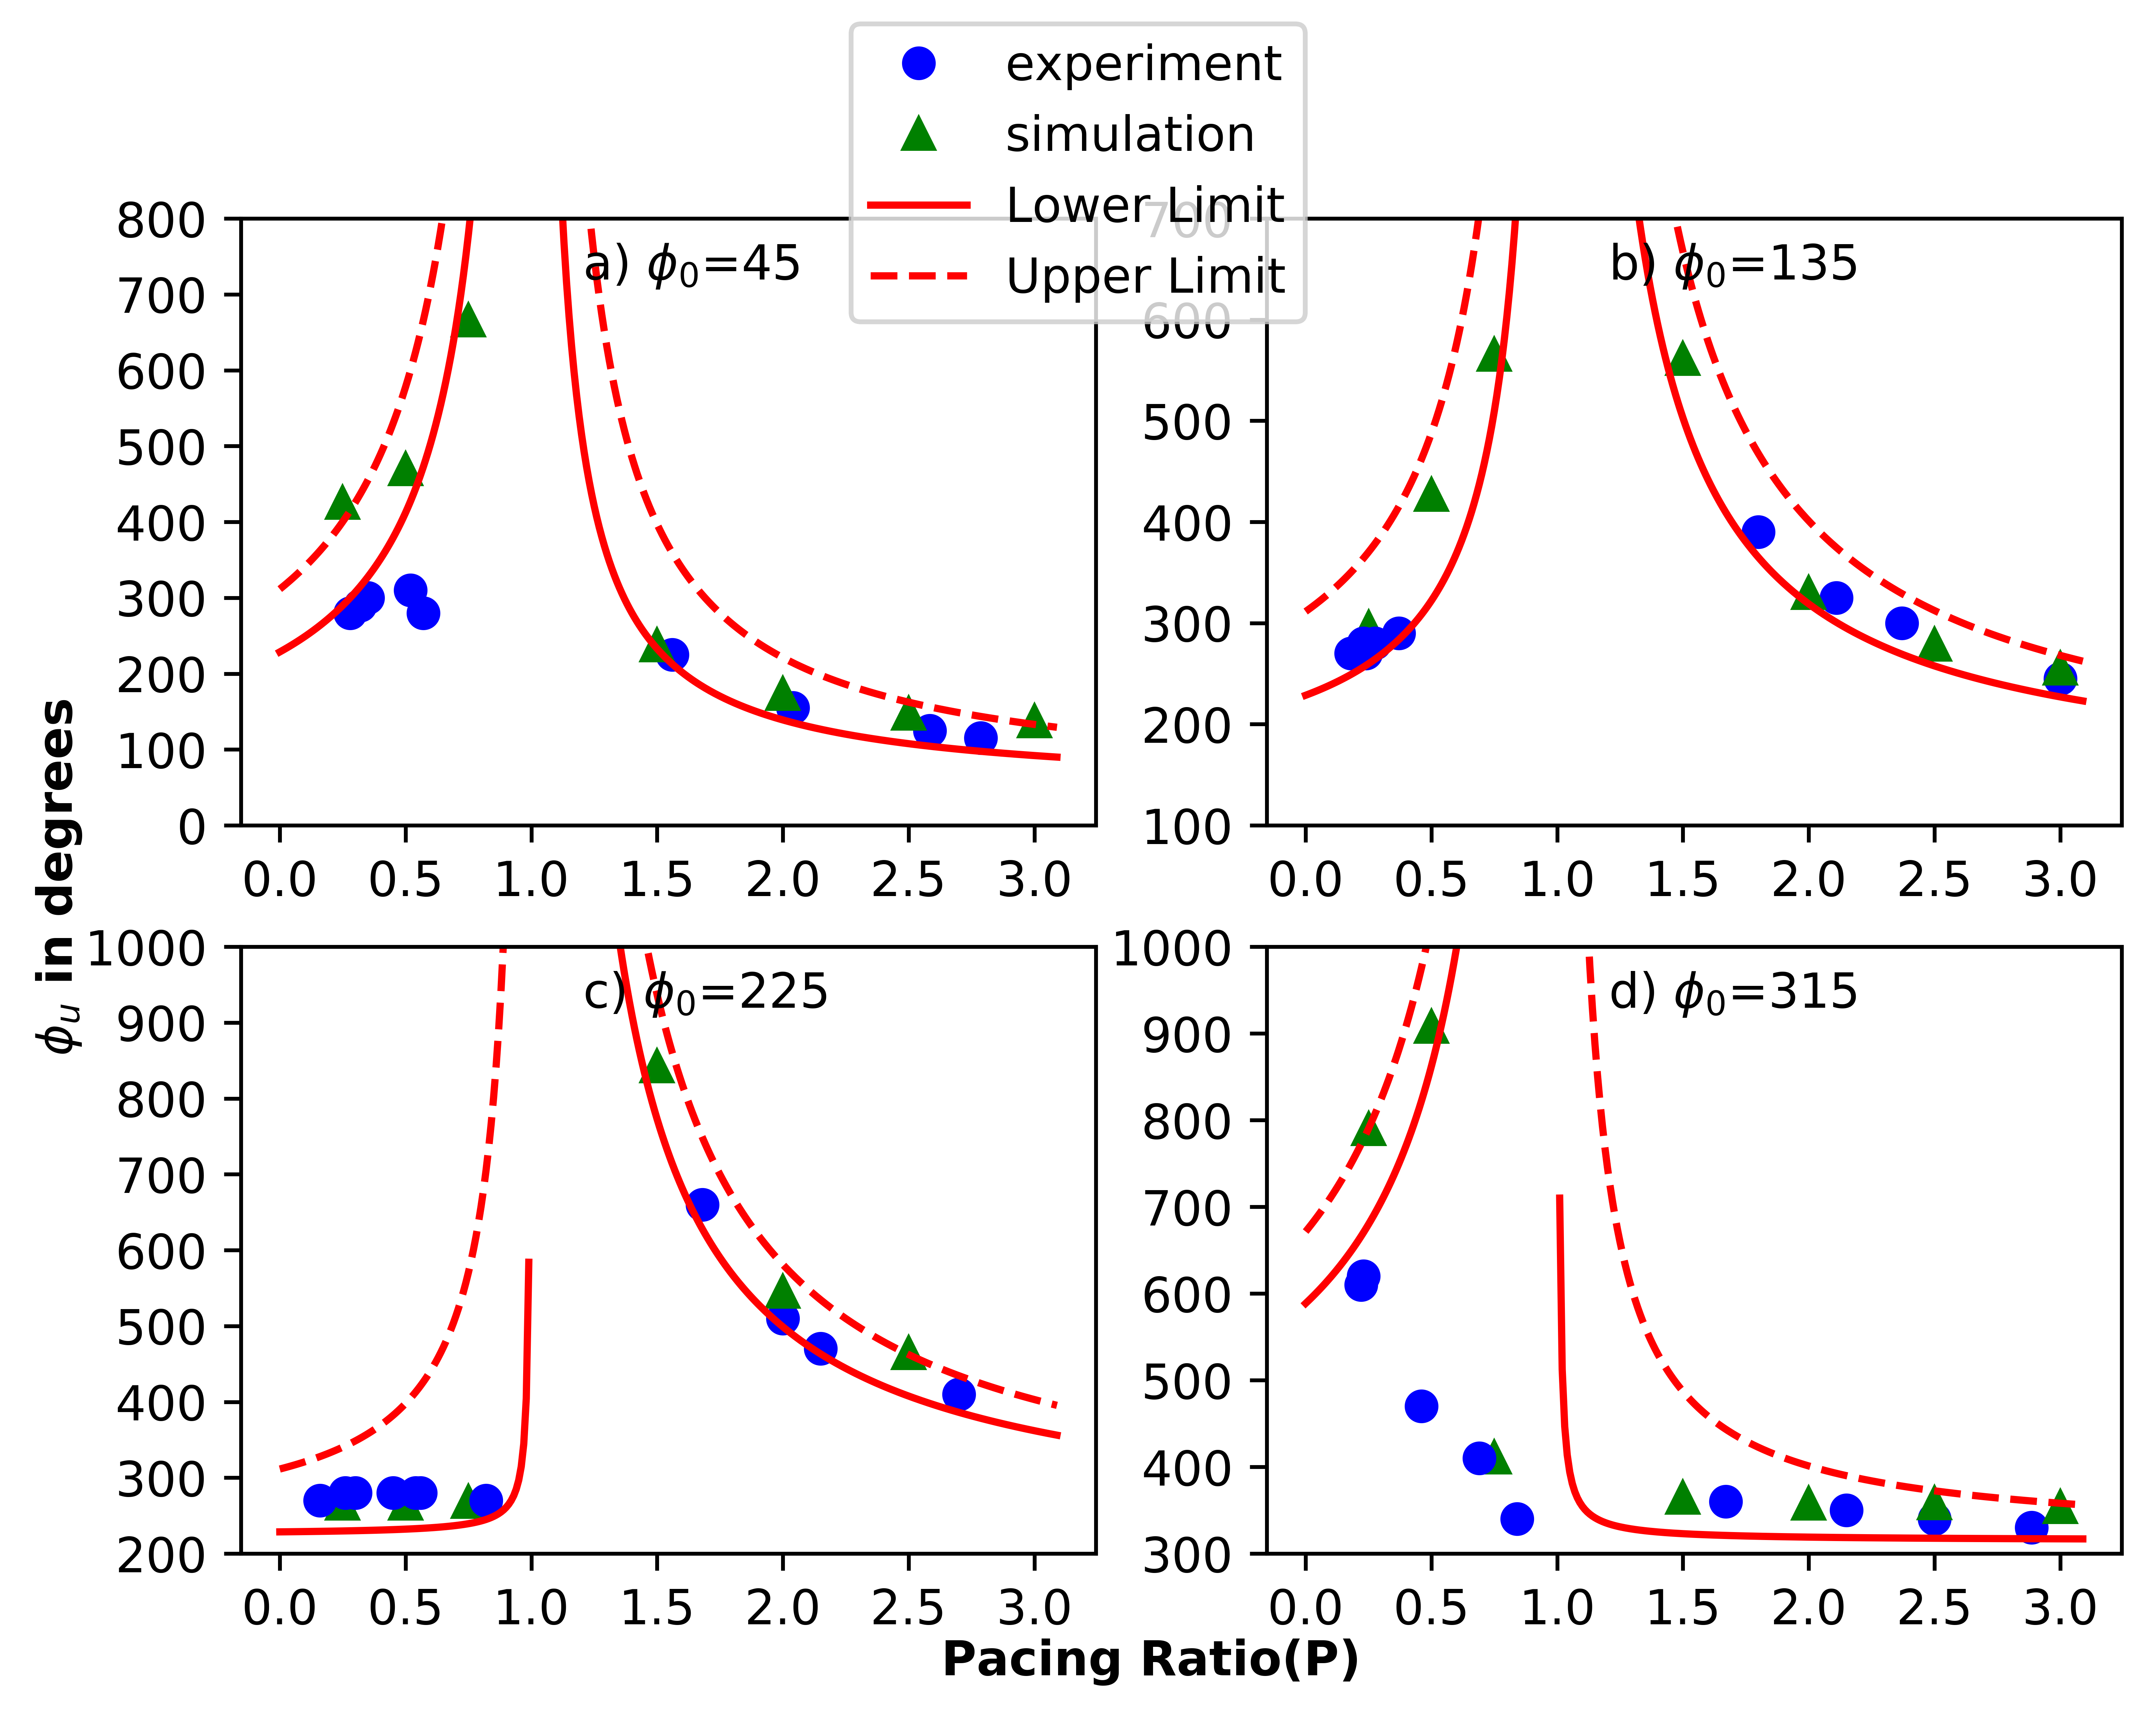
\includegraphics{E>Eth.png}
    \caption{Unpinning at $E>E_{th}$ 
    (${\sin^{-1}}{(\frac{E_{th}}{E})}=48.95^0$): Spiral waves with different ${\phi}_0$ are unpinned in a CPEF with both under-drive ($p<1$) and over-drive pacing ($p>1$). The solid bottom line represents the lower limit of the range of possible ${\phi}_u$-values given by the relation
    ${\phi}_u=(p{\phi}_0+48.95)/(p-1)$ for over-drive pacing and ${\phi}_u=(\pi-p{\phi}_0+48.59)/(1-p)$ for under-drive pacing. The upper limit of the range of possible ${\phi}_u$-values, given by the relation ${\phi}_u=(p{\phi}_0+\pi-48.95)/(p-1)$ for over-drive pacing and ${\phi}_u=(2\pi-p{\phi}_0-48.59)/(1-p)$ for under-drive pacing, are represented by the top dashed line. For ${\phi}_0 = 315^0$, the above equations must be added with $2\pi$ in order to get the positive phase values.
    Circles and triangles represent the experiment and simulation data respectively. 
    }
    \label{fig:unpinning_E>Eth}
\end{figure}
%
\begin{figure}[H]
    \centering
    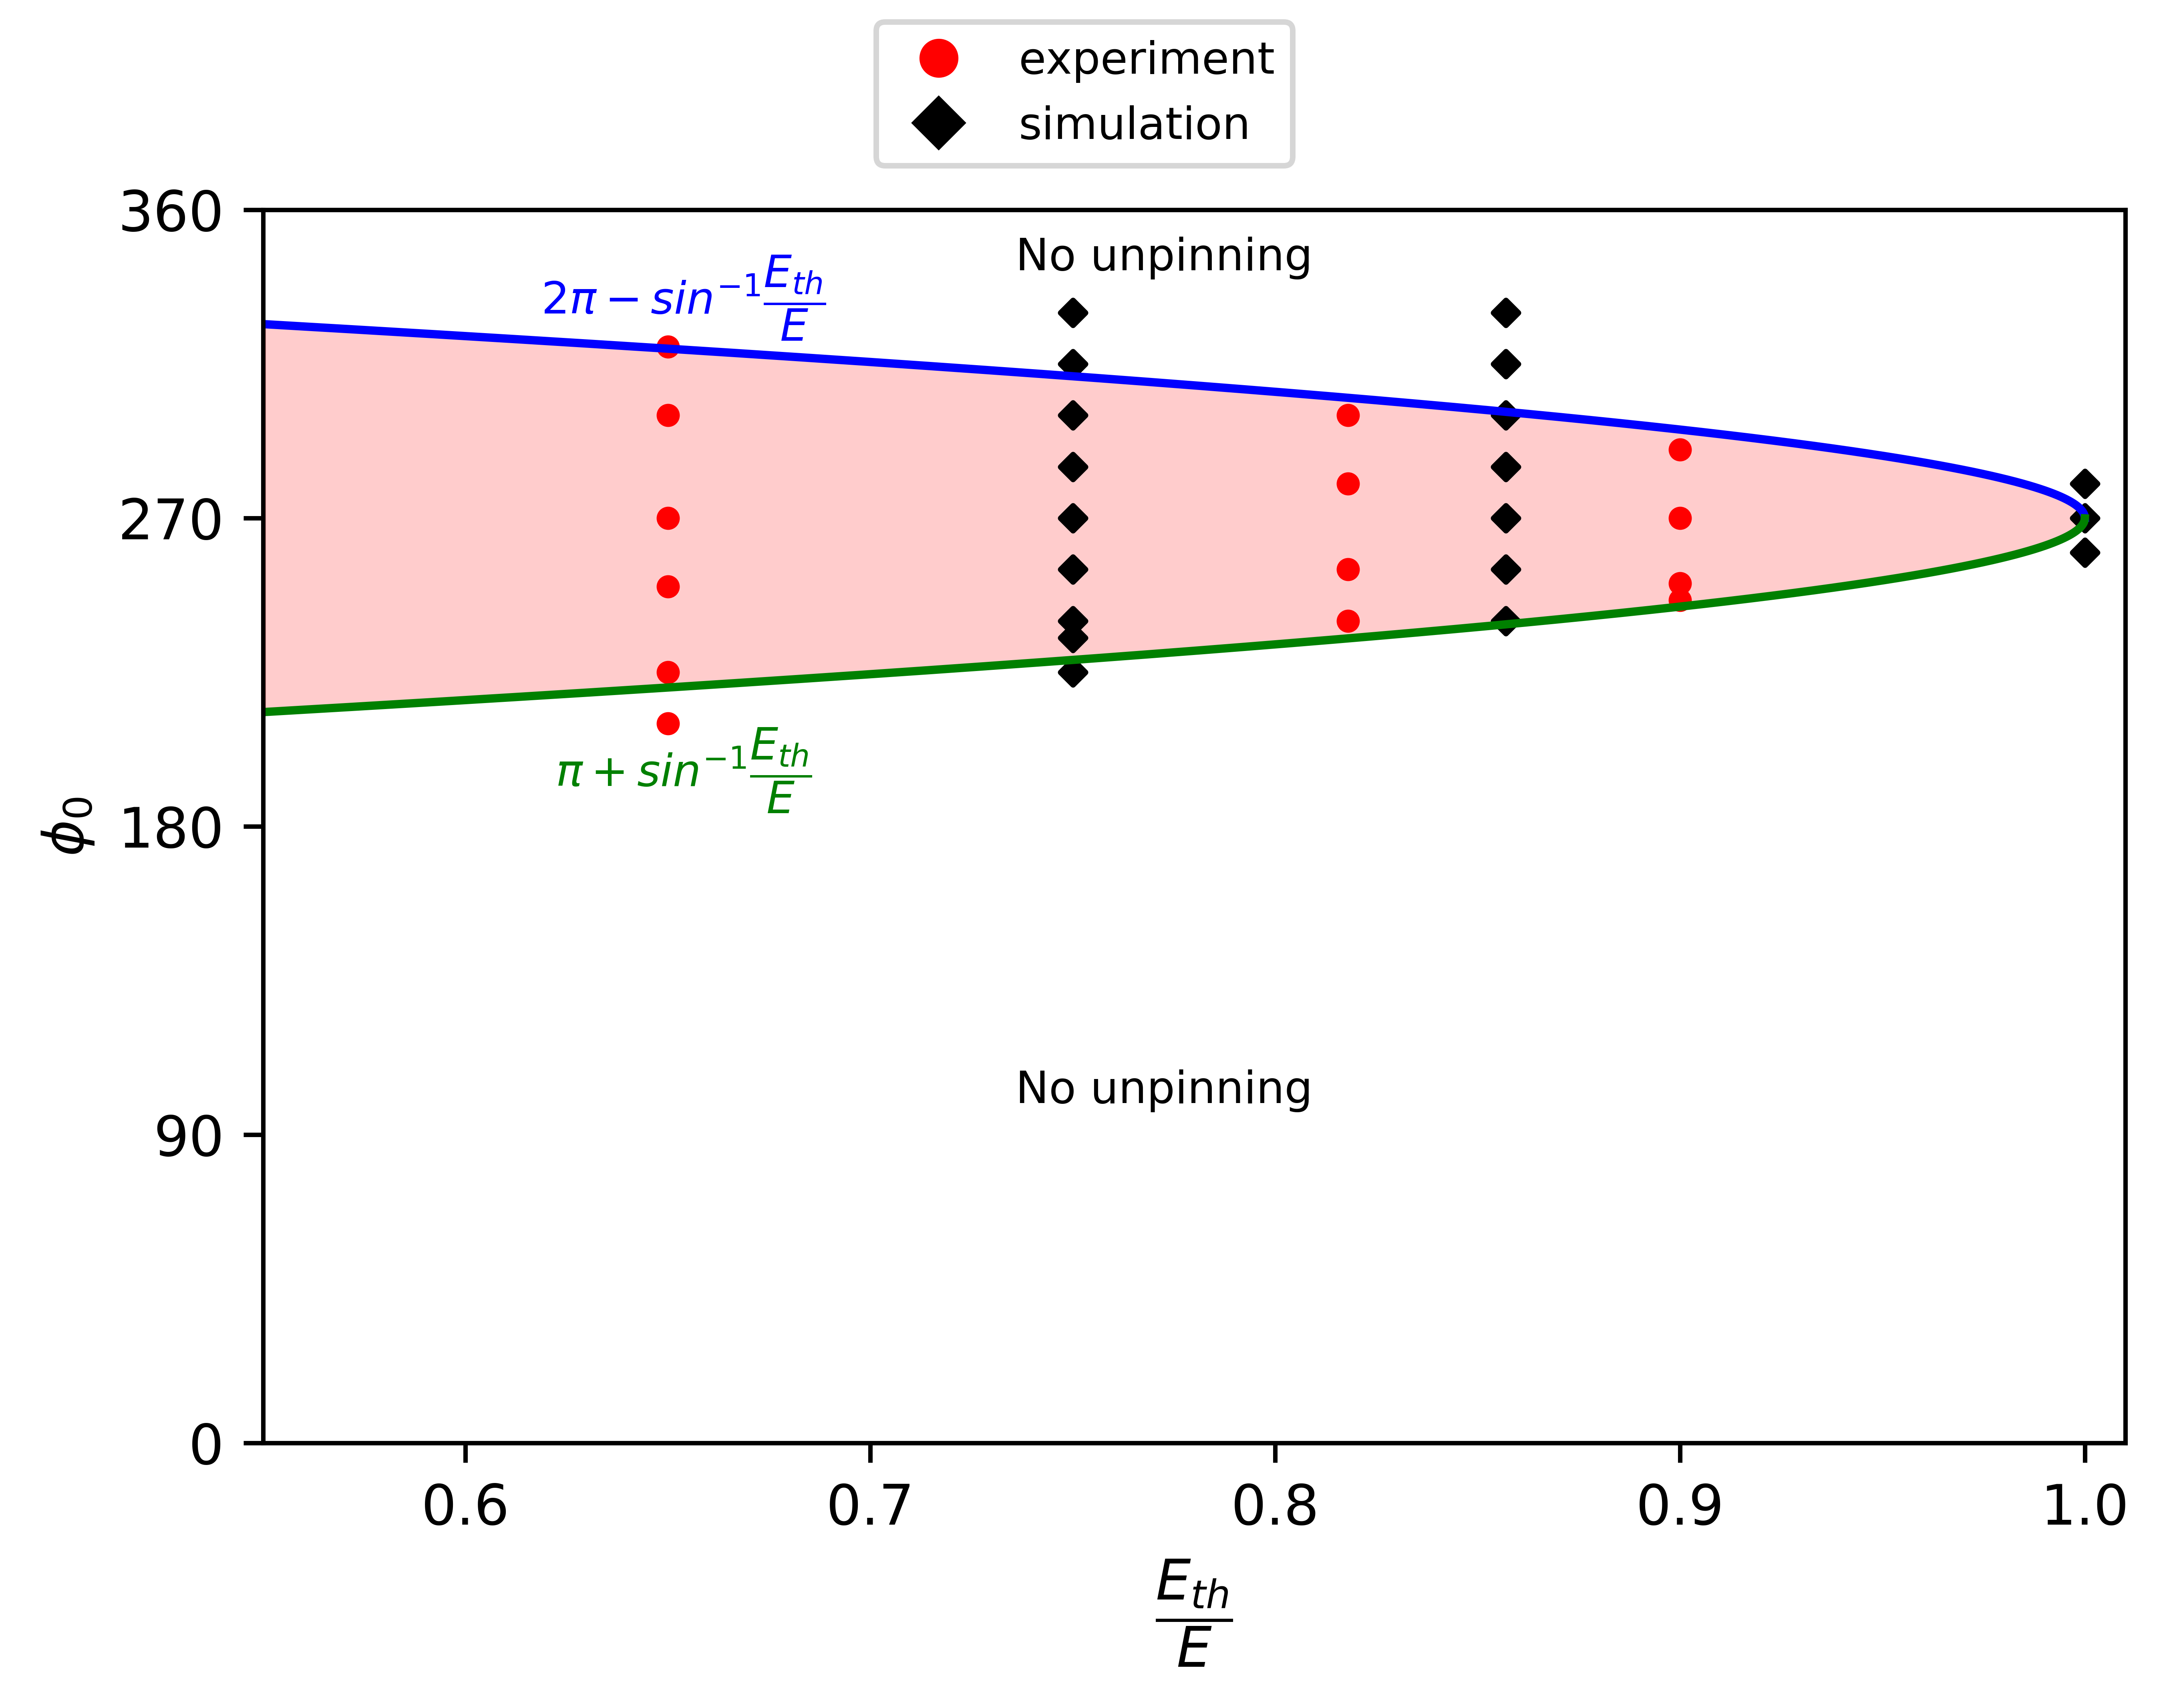
\includegraphics{p1.png}
    \caption{Unpinning of spiral wave with pacing ratio, p = 1 for different field strength: $\pi+{\sin^{-1}}{(\frac{E_{th}}{E})}$ and $2\pi-{\sin^{-1}}{(\frac{E_{th}}{E})}$ are the lower and upper limit of 
    the range of possible ${\phi}_0$-values which gives successful unpinning for p = 1. Shaded region corresponds to the cases of successful unpinning.
    Circles and diamonds represent the experiment and simulation data respectively.}
    \label{fig:unpinning_p1}
\end{figure}
%%%%%%%%%%%%%%%%%%%%%%%%%%%%%%%%%%%%%%%%%%%%%%%%%%%%%%%%%%%%%%%%%%%%%%%%%%%%%%%%%%%%%%%%%%%%%%%%%%%%%%%%%%%%%
\fi
Fig.\ref{fig:E_p1}a shows the unpinning phase window at $E>E_{th}$ for a fixed initial phase $\phi_0 = 225^0$. Here, the solid lines correspond to the lower limit, and the dashed lines correspond to the upper limit of the window according to the equations \ref{eq:overdrive} and \ref{eq:underdrive}. The unpinning always happens at a phase within this range immediately after the required interaction between the spiral and the field. In a DC field, 

%\subsection{p=1}
If the time period of applied CPEF $T_E$ = $T_s$, the pacing ratio will be p = 1. Here the spiral and the CPEF would rotate with a fixed phase difference. According to the equations for $\phi_u$, p = 1 will give infinity. It means that unpinning is impossible for p = 1. But in experiments and simulations, we have observed unpinning with this condition, but only for particular values of $\phi_0$ as marked in figure.\ref{fig:E_p1}b. 

For p = 1, unpinning happens only if the following condition is satisfied.
\begin{equation}
\pi+ \sin^{-1}(\frac{E_{th}}{E})  \leq \phi_0 \leq 2\pi-\sin^{-1}(\frac{E_{th}}{E})
\label{eq:p=1}
\end{equation}
This condition is reduced from the equations (\ref{eq:overdrive}) and (\ref{eq:underdrive}) by equating the numerator to zero. The observed $\phi_0$ falls within the limits of Arnold tongue's-shaped diagram (figure.\ref{fig:E_p1}b) given by equation.(\ref{eq:p=1}).
The width of the possible $\phi_0$-values which results in unpinning is $\Delta\phi_0 = \pi - 2 \sin^{-1}(\frac{E_{th}}{E})$. At E = $E_{th}$, $\Delta\phi_0 = 0$ and only spirals with $\phi_0 = 270^0$ unpins. For $E > E_{th}$, the unpinning is possible for a larger $\Delta\phi_0$, with a maximum value of $\pi$.  
From the figure.\ref{fig:E_p1}a and \ref{fig:E_p1}b, it is clear that a decrease in the value of $\frac{E_{th}}{E}$ for a fixed $E_{th}$ increases the possibility of unpinning.




%%%%%%%%%%%%%%%%%%%%%%%%%%%%%%%%%%%%%%%%%%%%%%%%%%%%%%%%%%%%%%%%%%%%%%%%%%%%%%%%%%%%%%%%%%%%%%%%%%%%%%%%%%%
\vspace{5pt}
\hrule
\vspace{5pt}
\textbf{Conclusions}

The electric force induces retardation in the propagation of a pinned spiral, which eventually leads to the unpinning of the spiral if the field possesses a threshold amplitude. 
The migration of negative bromide ions towards the anode causes a slowdown in the wave speed during the cycle of spiral rotation towards the cathode.
For any field strength greater than the threshold, the unpinning occurs when the electric field component along the tangential direction of spiral propagation reaches the critical threshold.
The unpinning demands a minimum interaction between the spiral and the field vector in an alignment in which the anode follows the spiral tip.
$\phi_u$ always comes within the unpinning phase window predicted by the mathematical conditions for any field strength greater than the threshold. Unpinning happens at a spiral phase, which comes immediately after the required interaction between the spiral and the field.
According to the equations, $\phi_u$ depends on p, E and $\phi_0$. These parameters fundamentally affect the interaction between the field vector and the spiral. 
Unpinning is possible for CPEF with underdrive pacing and p = 1 for a particular range of $\phi_0$. To get unpinning for p = 1, the initial position of the spiral must be ahead of the anode as obtained from equation.\ref{eq:p=1}.  The variations in $\phi_0$ with $\frac{E_{th}}{E}$ give an Arnold tongue's shaped diagram. 

The presence of mobile ions in the BZ reaction causes the excitation waves in the medium to respond uniquely with an applied electric field. A systematic study of this interaction will provide new insights into the control and applications of the chemical waves.

\iffalse
The field-induced motion of $Br^-$ ions in the BZ reaction forces the core of a free spiral to drift toward the anode. An equivalent electric force induces retardation in the propagation of a pinned spiral, which eventually leads to its unpinning and a further drift similar to that of a free spiral. The retarding electric force can drag the spiral wave and cause unpinning only if it possesses a threshold amplitude. 
For any field strength greater than the threshold, the unpinning occurs when the electric field component along the tangential direction of spiral propagation reaches the critical threshold. This assumption leads to the deduction of conditions for the unpinning phase window.
According to this, the quantities pacing ratio, initial spiral phase, and field strength provide sensitive control over unpinning. It is interesting to notice the unpinning with an electric field of lower frequency than the spiral wave in the BZ reaction. Unpinning is also possible for a unit pacing ratio with a particular set of initial phases. 

It is evident from the study that the process of unpinning is not instantaneous with the application of the field. Instead, it requires a minimum duration of interaction between the spiral and the field, which is decided by other parameters such as the pacing ratio, initial spiral phase, and field strength.
The presence of mobile ions in the BZ reaction causes the excitation waves in the medium to respond uniquely with an applied electric field. A systematic study of this interaction will provide new insights into the control and applications of the chemical waves.
\fi


\begin{acknowledgments}

\end{acknowledgments}

\section{Author Contributions}
S.V.A and T.K.S planned the objectives of the study. S.V.A performed the experiments. P.S built the experimental setup. S.P designed the numerical study as well as the computational framework. A.S performed numerical simulations. A.S and T.K.S formulated the equations. S.V.A and A.S collected and analysed the data with help from T.K.S. S.V.A and T.K.S wrote the paper. All authors helped to edit the paper. 


\appendix
\iffalse
\section{Unpinning of a CW spiral}

\begin{figure}[H]
    \centering
    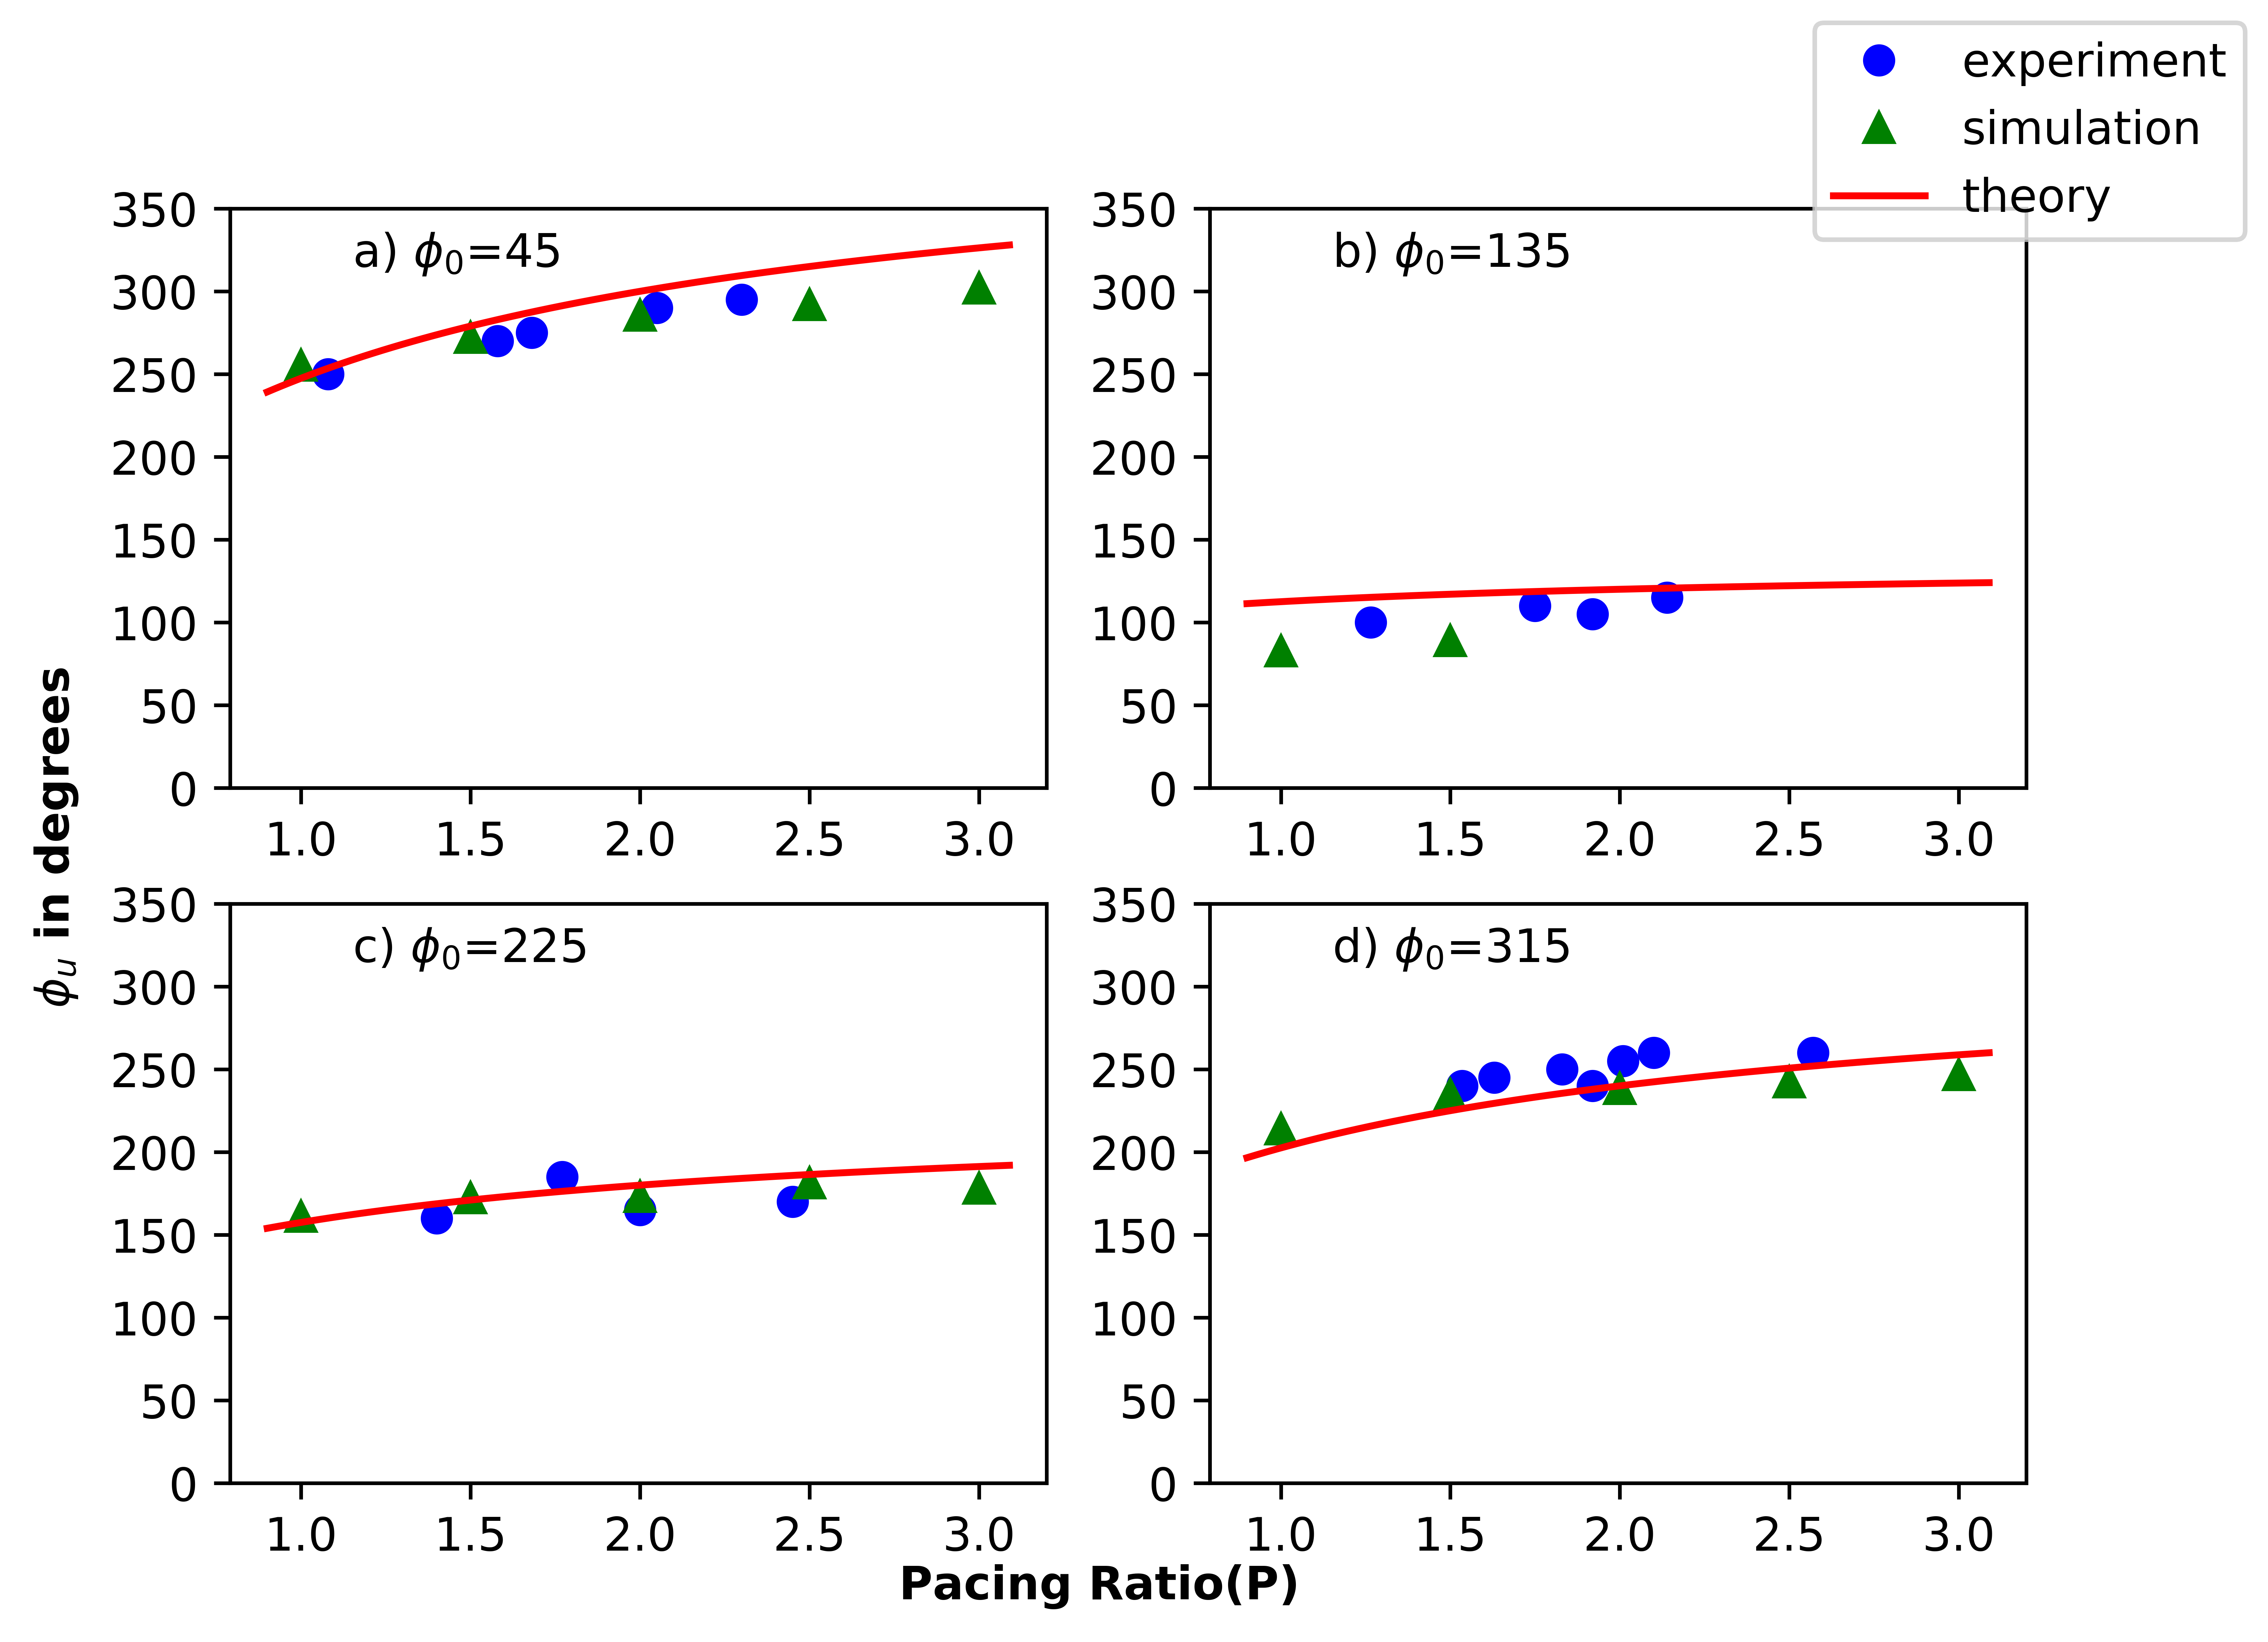
\includegraphics{appendix_cw_Eth.png}
    \caption{E=Eth}
    \label{fig:unpinning_cw}
\end{figure}
%%%%%%%%%%%%%%5 CW equation
at E=$E_{th}$
\begin{equation}
    \phi_{u} = \frac{\phi_{0}+\frac{1}{p}{\sin^{-1}} (\frac{E_{th}}{E})}{1+\frac{1}{p}}
    \label{eq:basic_eqn_cw}
\end{equation}
\centering or 
\begin{equation}
    \phi_{u} = \frac{2\pi+\phi_{0}+\frac{1}{p}{\sin^{-1}} (\frac{E_{th}}{E})}{1+\frac{1}{p}}
    \label{eq:basic_eqn_cw}
\end{equation}
\fi


%%%%%%%%%%%%%%%Comparison
\section{Comparison between numerical models and between pinning obstacles of different geometry}

\begin{figure}[H]
    \centering
    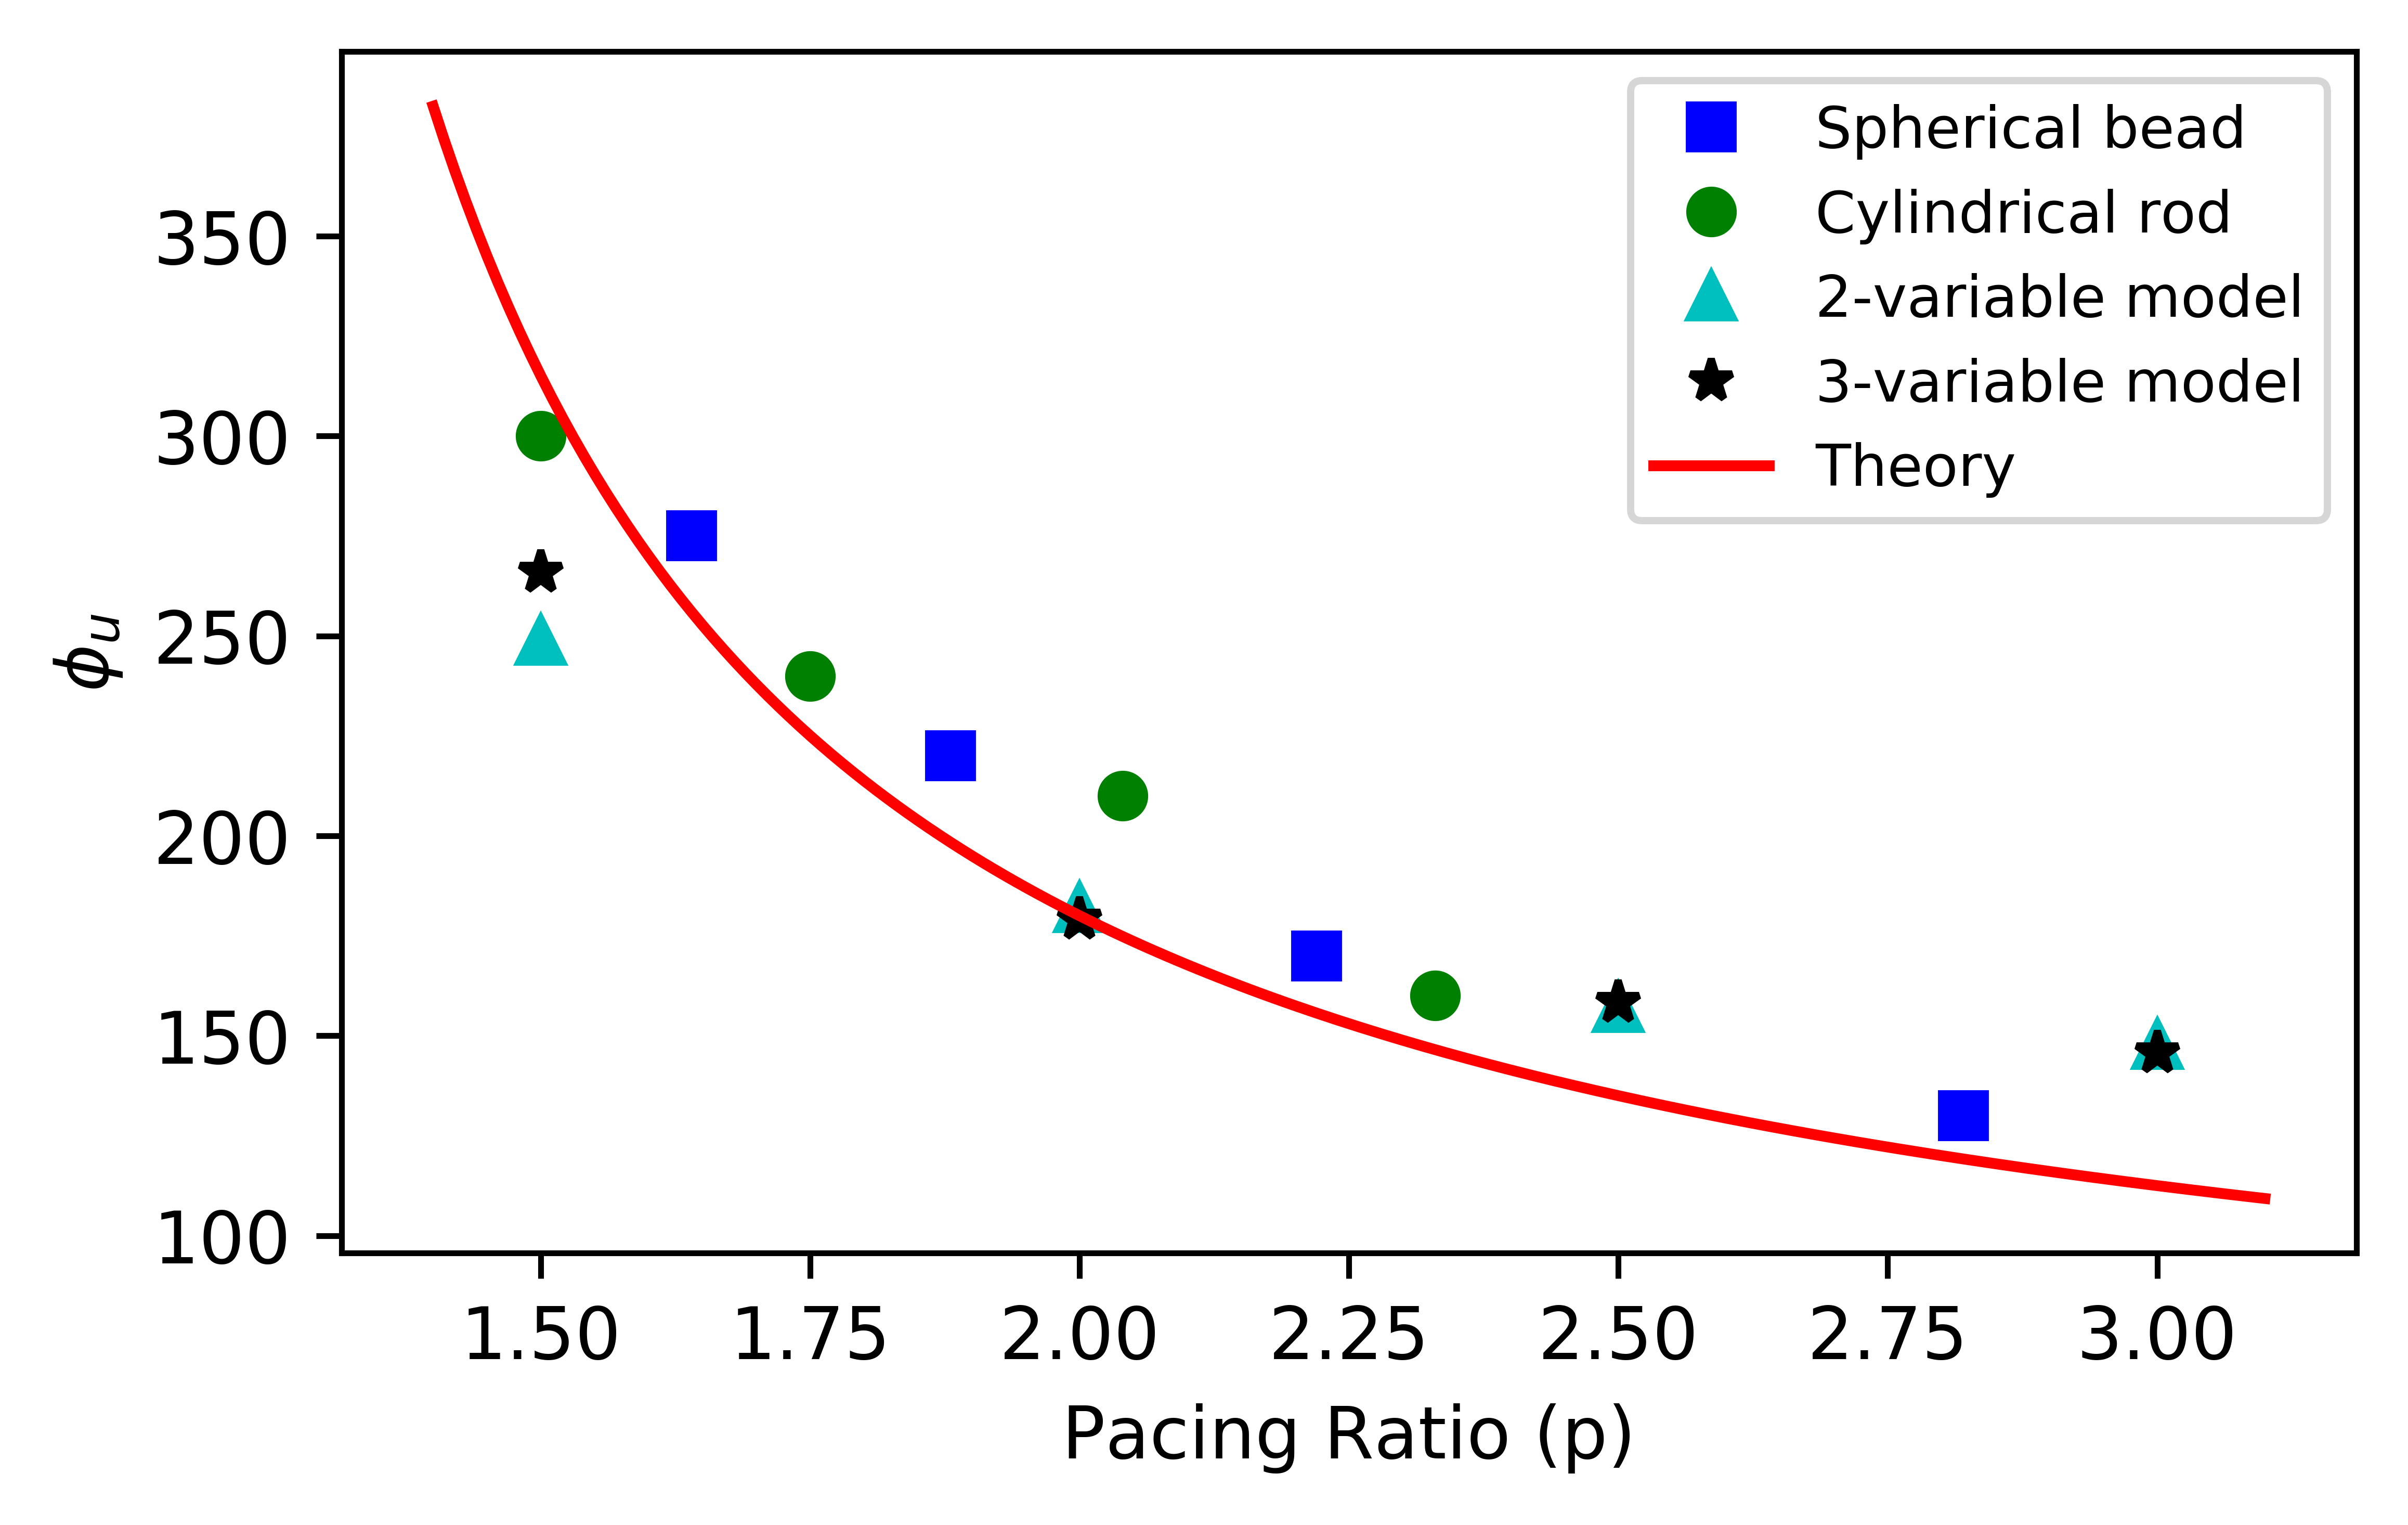
\includegraphics{appendix_23oregonator_beadrod.png}
    \caption{Caption}
    \label{fig:unpinning_comparison}
\end{figure}


\nocite{*}

\bibliography{ref}% Produces the bibliography via BibTeX.

\end{document}
%
% ****** End of file apssamp.tex ******

\subsection{Overdrive pacing}

\begin{equation}
\frac{p \phi_0+ {\sin^{-1}}(\frac{E_{th}}{E})}{p-1}   \leq \phi_u \leq \frac{p \phi_0+\pi -{\sin^{-1}}(\frac{E_{th}}{E})}{p-1}
\end{equation}

\subsection{ Underdrive pacing}

\begin{equation}
\frac{\pi+ {\sin^{-1}}(\frac{E_{th}}{E})-p \phi_0}{1-p}   \leq \phi_u \leq \frac{2\pi-p \phi_0-{\sin^{-1}}(\frac{E_{th}}{E})}{1-p}
\end{equation}
